%  MDPI Materials article — populated from the official template (ACS numbered references)
%  Compile: place in the MDPI template folder (with Definitions/), then run:
%     pdflatex main -> bibtex main (if external .bib) -> pdflatex main x2
%  Or upload the whole folder to Overleaf (it compiles as-is).
%=================================================================
\documentclass[materials,article,submit,pdftex,moreauthors]{Definitions/mdpi}

% Fallback for template commands not defined by this mdpi.cls version
\providecommand{\TitleCitation}[1]{}
\providecommand{\AuthorCitation}[1]{}

% Full-page landscape floats for the dense bibliometric figures
\usepackage{rotating}

\firstpage{1}
\makeatletter
\setcounter{page}{\@firstpage}
\makeatother
\pubvolume{1}
\issuenum{1}
\articlenumber{0}
\pubyear{2026}
\copyrightyear{2026}
\datereceived{ }
\dateaccepted{ }
\datepublished{ }

\Title{Interpretable Machine Learning for One-Part Fly-Ash/Slag Geopolymer Strength Prediction: Toward Multifunctional Binder Design}

\TitleCitation{Interpretable Machine Learning for One-Part Geopolymer Strength Prediction}

\newcommand{\orcidauthorA}{0000-0000-0000-0000}
\newcommand{\orcidauthorB}{0000-0000-0000-0000}
\newcommand{\orcidauthorC}{0000-0000-0000-0000}

\Author{Vinoth Nageshwaran $^{1,}$*\orcidA{}, Sudhir Amritphale $^{2}$\orcidB{} and Soundararajan Ezekiel $^{3}$\orcidC{}}

\AuthorNames{Vinoth Nageshwaran, Sudhir Amritphale and Soundararajan Ezekiel}

\address{%
$^{1}$ \quad School of Computer and Information Sciences, University of the Cumberlands, 6178 College Station Drive, Williamsburg, KY 40769, USA\\
$^{2}$ \quad Alchemy Geopolymer Solutions, Ruston, LA 71270, USA\\
$^{3}$ \quad Department of Mathematical and Computer Sciences, Indiana University of Pennsylvania, Indiana, PA 15705, USA}

\corres{Correspondence: vnageshwaran41452@ucumberlands.edu}

\abstract{Portland cement production accounts for roughly 8\% of anthropogenic CO\textsubscript{2} emissions, driving interest in low-carbon geopolymer binders. One-part (``just-add-water'') geopolymers, which replace hazardous liquid activators with a dry, pre-blended solid activator, are especially suited to field deployment where handling safety and logistics are decisive. However, their formulation space is combinatorially vast, and trial-and-error development cannot efficiently navigate it. This paper reviews one-part geopolymer science, presents a new comparative and interpretable ML analysis of a published 80-mixture one-part fly-ash/GGBS geopolymer dataset from twelve studies, and proposes an AI-assisted design framework. The ML demonstration targets 28-day compressive strength only. Under leave-one-source-out (LOSO) cross-validation---the appropriate test for a literature-pooled dataset---gradient-boosted trees achieved R\textsuperscript{2} = 0.61, well above a linear baseline (0.36), suggesting that non-linear structure transfers across studies; a random split gives a higher but less reliable R\textsuperscript{2} = 0.90 on only 16 test mixtures. Because fly-ash and GGBS contents are near-perfectly anti-correlated ($r = -0.99$), we model the precursor axis as a single slag-fraction descriptor; SHAP then identifies this precursor balance and the activator's Na\textsubscript{2}O dosage as the dominant, mechanistically coherent strength levers. Demonstrated for strength, the framework offers a transferable route toward multifunctional low-carbon binders for protective and infrastructure applications.}

\keyword{one-part geopolymer; machine learning; alkali-activated materials; multifunctional composites; mix design optimization; defense infrastructure}

\begin{document}

\section{Introduction}
Concrete is the most-consumed manufactured material on Earth, and the ordinary Portland cement (OPC) that binds it is responsible for approximately 8\% of global anthropogenic carbon dioxide emissions---a share arising from both the calcination of limestone and the fossil energy required to reach clinkering temperatures. As national decarbonization commitments tighten and as the construction sector confronts the scale of its embodied-carbon footprint, the search for binders that deliver OPC-comparable mechanical performance at a fraction of the emissions has become one of the defining materials challenges of the coming decades. Alkali-activated materials (AAMs) and geopolymers---synthesized by reacting aluminosilicate precursors such as fly ash, ground granulated blast-furnace slag (GGBS), or metakaolin with an alkaline activator---are the most technologically mature low-carbon binder class, capable of 40--80\% reductions in cradle-to-gate CO\textsubscript{2} relative to OPC while reusing industrial by-products that would otherwise be landfilled.

Despite three decades of research, conventional "two-part" geopolymers face a persistent barrier to field adoption: they require a concentrated liquid alkaline activator, typically a sodium or potassium hydroxide/silicate solution. These solutions are corrosive, viscous, exothermic on preparation, and hazardous to handle, and they cannot be dry-bagged, shipped, and stored like OPC. This constraint is disqualifying precisely in the settings where a rapidly deployable, low-carbon, high-performance binder would be most valuable---forward operating bases, disaster-response reconstruction, remote infrastructure, and protective structures---where trained personnel, controlled mixing environments, and hazardous-materials logistics are unavailable. The activator, in short, is the bottleneck standing between geopolymer science and field practice.

One-part, or "just-add-water," geopolymers dissolve this bottleneck. By pre-blending a solid activator---commonly anhydrous sodium metasilicate, sodium aluminate, or a calcined/mechanochemically activated alkali source---with the aluminosilicate precursor into a single dry powder, the one-part approach reproduces the OPC use-model exactly: the end user adds only water. This transfers all hazardous chemistry upstream into a controlled manufacturing facility and yields a shelf-stable, transportable binder amenable to bagging, spraying, and even 3D printing in the field. Since the foundational demonstrations of ambient-cured one-part mixes in the mid-2010s~\cite{ref13,ref23}, the sub-field has grown rapidly, with formulations now spanning fly-ash, slag, red-mud, and natural-pozzolan precursors~\cite{ref14,ref15} and functional variants including fibre-reinforced, engineered-cementitious, foamed, and printable composites~\cite{ref19,ref21,ref22}.

Yet this very versatility creates a design problem. The performance of a one-part geopolymer is governed by a high-dimensional, strongly interacting formulation space: precursor identity and blend ratio, solid-activator type, dosage, and silica modulus, water-to-binder ratio, functional additives (fibres, fillers, conductive or shielding phases), and curing regime. These variables interact non-linearly---the optimal activator dosage depends on precursor reactivity; the benefit of heat curing depends on the fly-ash/slag balance; workability, strength, and durability trade against one another. The combinatorial size of this space defeats the one-factor-at-a-time experimentation that still dominates the literature, and it explains why property optimization in one-part systems remains slow, sample-hungry, and poorly transferable between laboratories.

Machine learning (ML) offers a direct response to this challenge. Over the past five years, data-driven models---artificial neural networks, tree ensembles, support vector machines, and gene-expression programming---have been applied with growing success to predict the compressive strength and, less often, the durability and fresh-state properties of alkali-activated concretes~\cite{ref1,ref2,ref3,ref8}, and interpretability methods such as SHAP (SHapley Additive exPlanations) are beginning to convert these models from black-box predictors into sources of design insight~\cite{ref25,ref38}. A bibliometric survey we conducted for this work (1,850 geopolymer papers, 2014--mid-2026; Section~\ref{sec:bibmethod}) confirms both the momentum and the gap: ML-assisted and one-part research are the two fastest-growing streams in the field, yet their explicit intersection remains a small, if rapidly growing, cluster of roughly two dozen papers concentrated in the last three years, and a concept co-occurrence analysis over paper abstracts shows the strongest ML associations running to compressive-strength prediction of conventional two-part mixes, with markedly weaker abstract-level coupling to one-part formulation and essentially none to fibre-reinforcement or thermal/functional performance. Machine learning has, in other words, only just begun to be turned on the one-part design problem, and scarcely at all on the multifunctional properties that defense and infrastructure applications demand.

This paper addresses that gap on three fronts. First, we review the materials science of one-part geopolymer composites---precursor and activator chemistry, reaction mechanisms, mechanical and durability behaviour, and the emerging multifunctional variants relevant to protective and civil infrastructure. Second, we present a new comparative and interpretable ML analysis of a \emph{published} 80-mixture one-part fly-ash/GGBS geopolymer dataset (compiled from twelve independent studies): the dataset is not new, but the comparative modelling, leave-one-source-out evaluation, and SHAP interpretation are. We train and compare four regression algorithms, evaluate them by both random-split and leave-one-source-out cross-validation, and apply SHAP analysis to extract design-actionable feature effects for the compressive-strength target. Third, we synthesize these threads into a generalizable, interpretable AI-assisted design framework that links mixture descriptors to multifunctional performance targets and closes the loop from data curation through model interpretation to experimental validation. Our aim is not a single optimized mix but a transferable methodology for the rational, accelerated design of the field-deployable low-carbon binders that defense and civil infrastructure increasingly require.

\begin{sidewaysfigure}
\centering
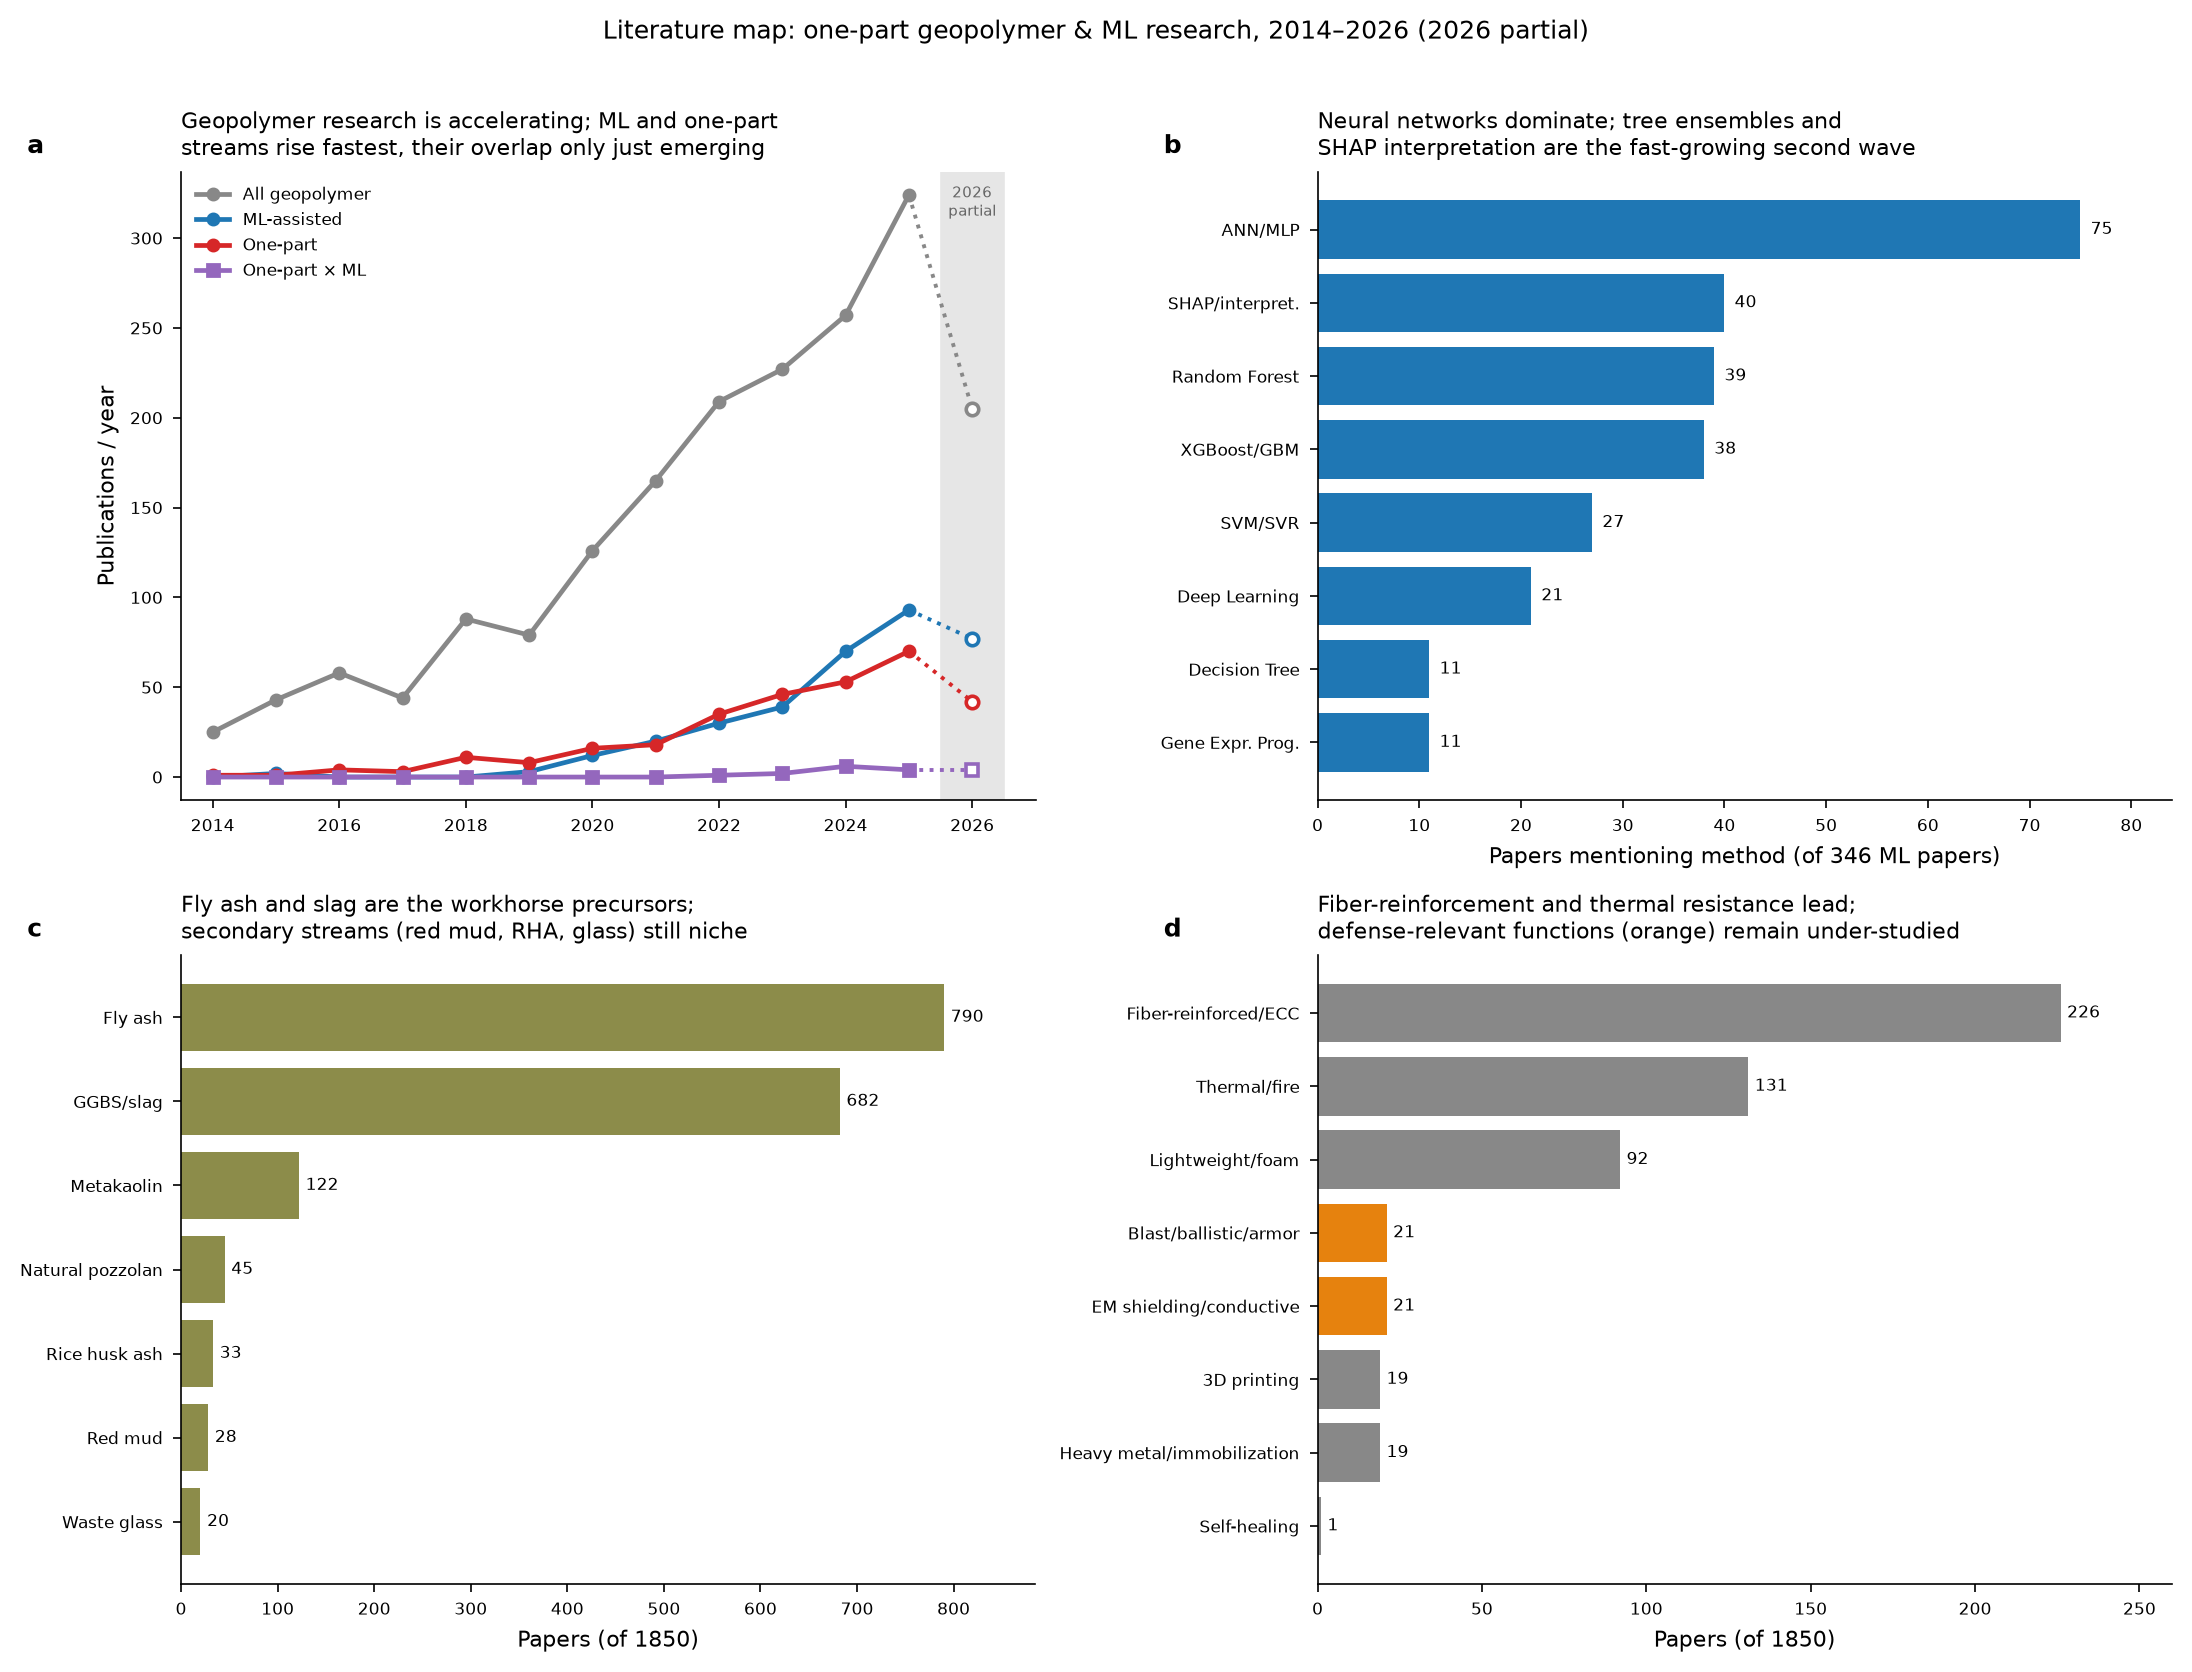
\includegraphics[width=0.86\textheight,height=\textwidth,keepaspectratio]{figures/figure1_literature_map.png}
\caption{Bibliometric landscape of the geopolymer field (2014--mid-2026, $n = 1850$). (\textbf{a}) Publication trends by sub-stream (2026 partial); (\textbf{b}) ML methods; (\textbf{c}) precursors; (\textbf{d}) functional themes. The one-part $\times$ ML intersection is a small but rapidly growing cluster concentrated in recent years.\label{fig1}}
\end{sidewaysfigure}

\begin{sidewaysfigure}
\centering
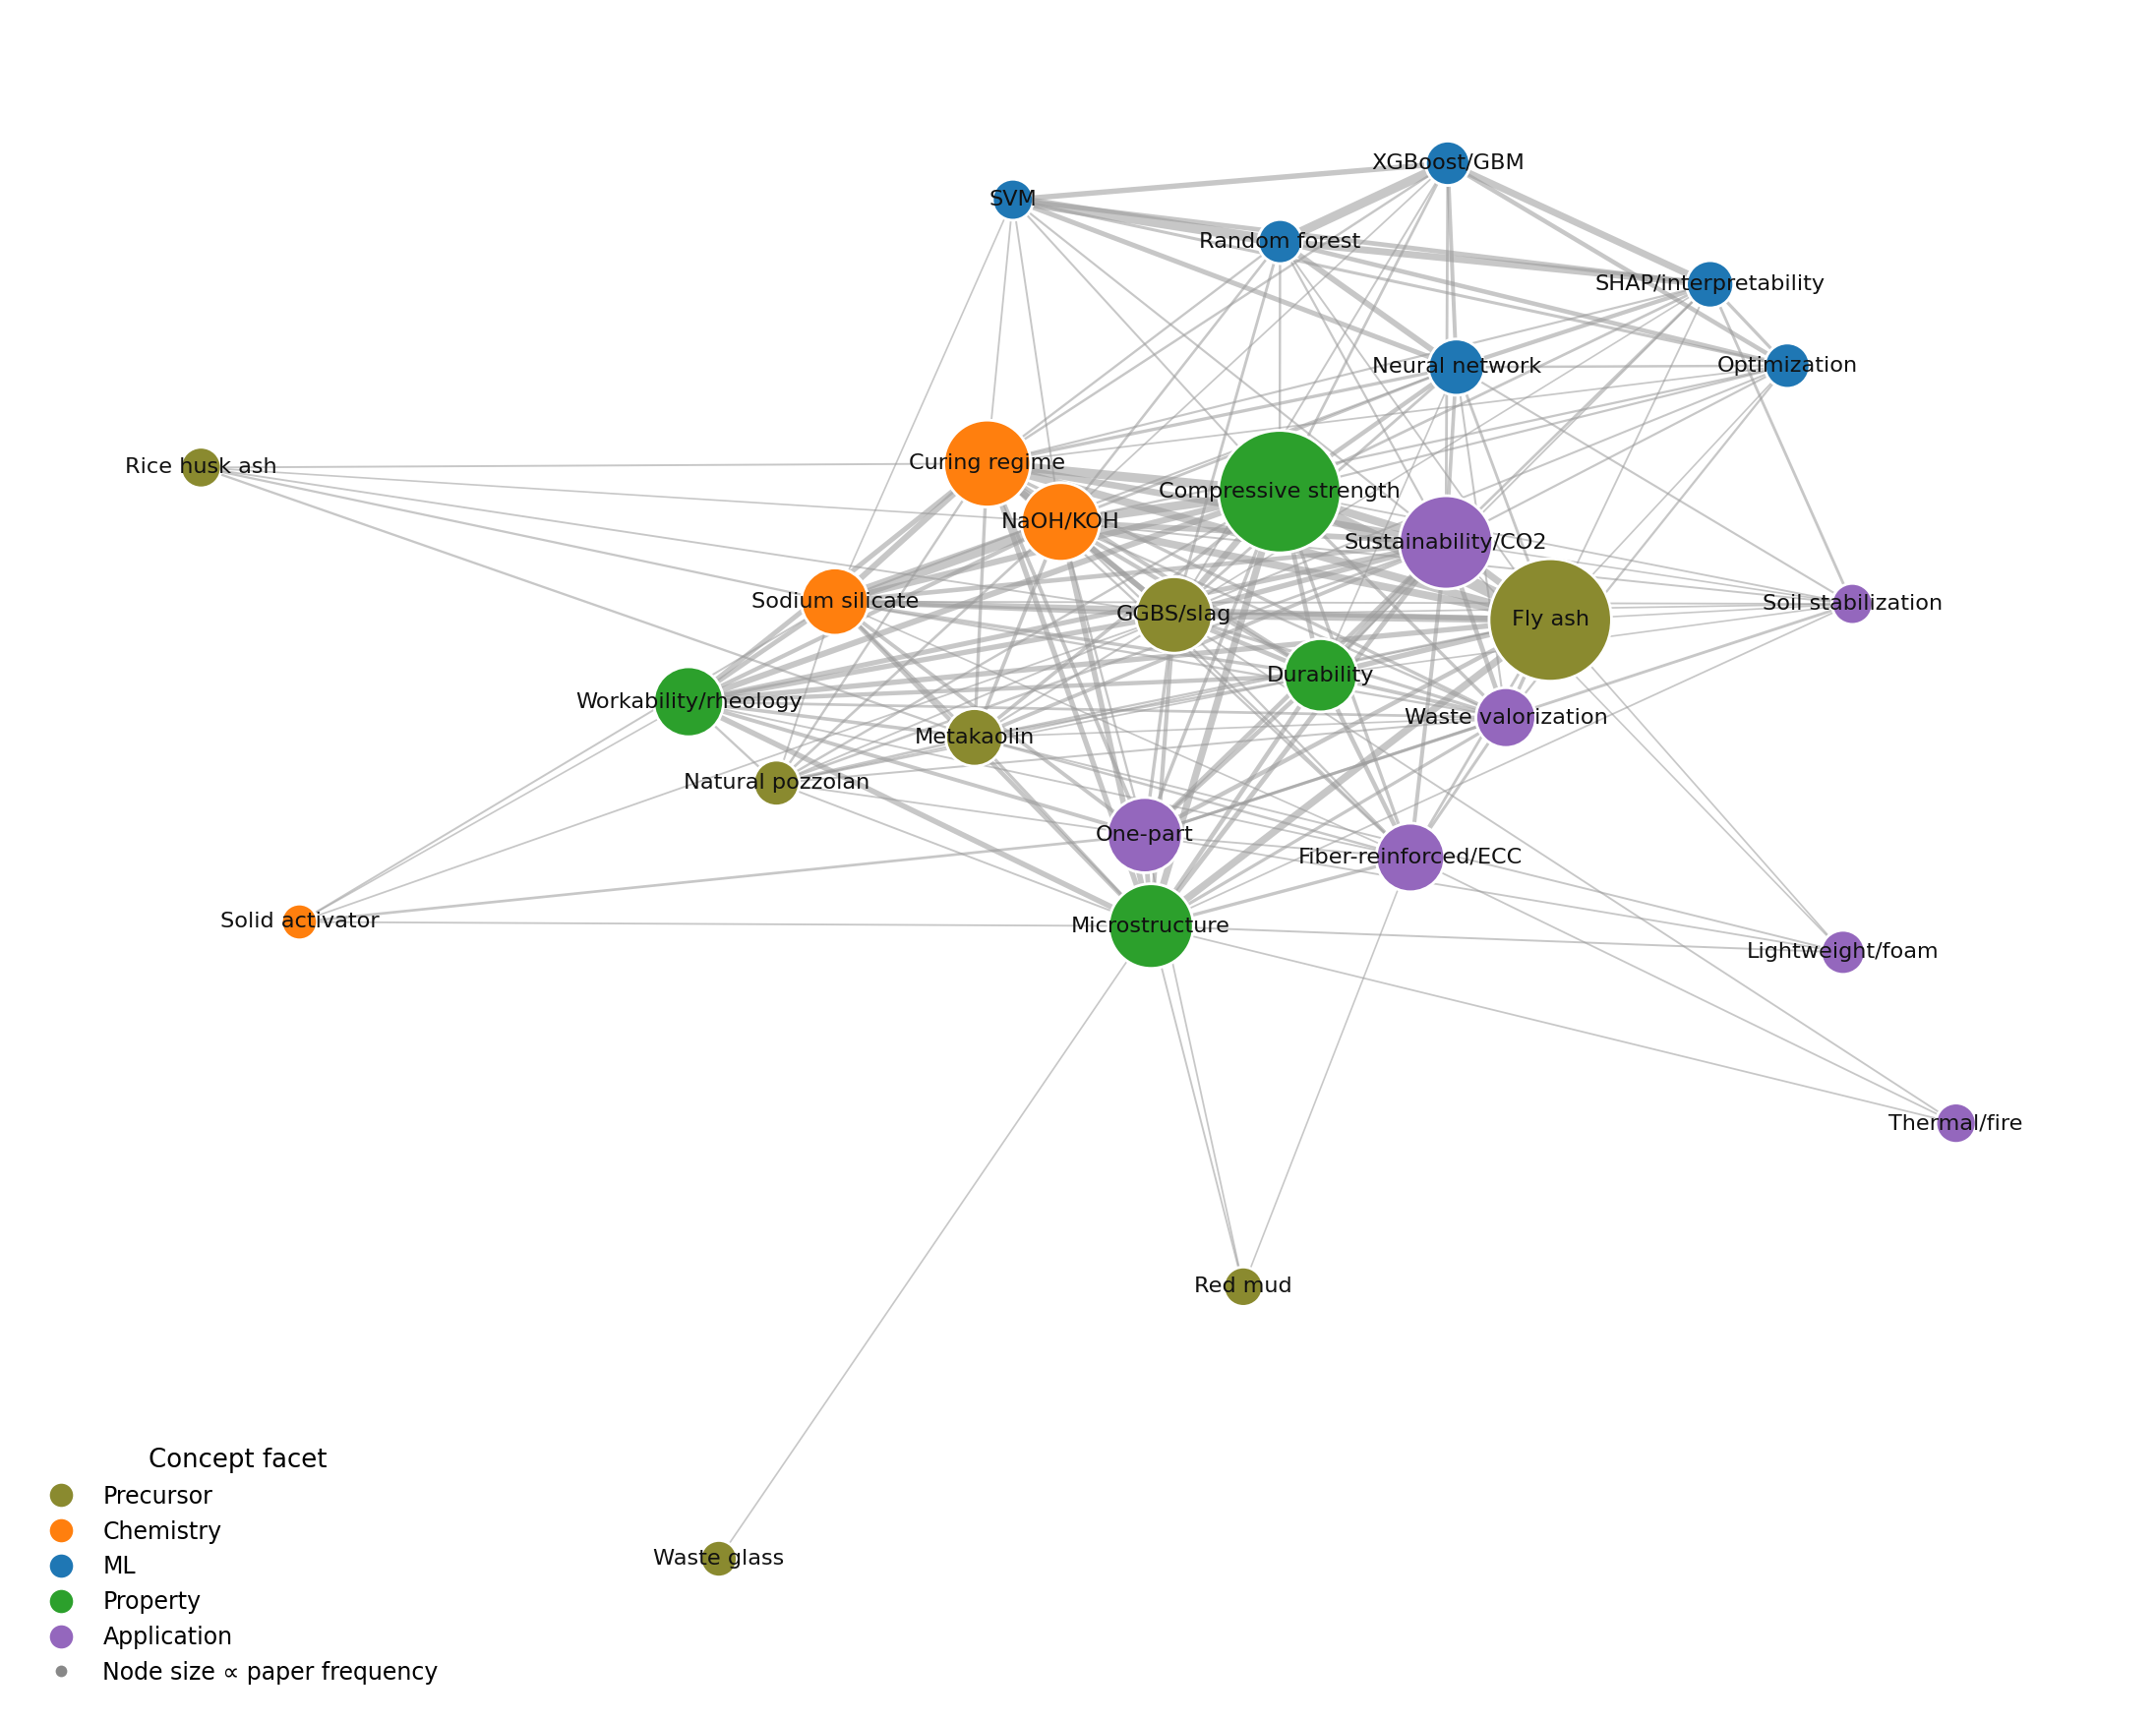
\includegraphics[width=0.86\textheight,height=\textwidth,keepaspectratio]{figures/figure2_concept_network.png}
\caption{Concept co-occurrence network of the corpus (1{,}092 papers with title text longer than 120 characters). Machine-learning methods (blue) cluster together and couple to the mix-design/strength core, but not to one-part formulation or multifunctional properties.\label{fig2}}
\end{sidewaysfigure}

\subsection{Bibliometric methodology}\label{sec:bibmethod}

\sloppy
The literature map in Figures~\ref{fig1}--\ref{fig2} was built from a reproducible query of the Crossref REST API, retrieved on 1 July 2026, filtered to \texttt{from-pub-date:2014-01-01,type:journal-article}, with cursor pagination (200 records per page). Eight \texttt{query.bibliographic} strings were issued: (1) ``geopolymer machine learning''; (2) ``one-part geopolymer''; (3) ``one-part geopolymer compressive strength''; (4) ``geopolymer concrete machine learning prediction''; (5) ``alkali activated material mix design optimization machine learning''; (6) ``geopolymer electromagnetic shielding OR fiber reinforced multifunctional''; (7) ``one-part alkali activated slag fly ash''; (8) ``geopolymer artificial neural network compressive strength''. Records were pooled and de-duplicated by DOI, yielding 4{,}312 unique articles.

Relevance and sub-stream tagging used case-insensitive regular expressions applied to the lower-cased, HTML-stripped title text of each record (the corpus retains title-level bibliographic metadata; abstracts were not stored). A record was retained as on-topic if it matched \texttt{geopolymer | alkali[- ]activat | geopolymeric}, reducing the pool to 1{,}850 papers spanning 2014 to mid-2026. The ML stream matched \texttt{machine learning | deep learning | neural network | random forest | gradient boost | xgboost | artificial intelligence | ann | svm | gep | ensemble model | predictive model | data[- ]driven | gene expression programming}; the one-part stream matched \texttt{one[- ]part | just[- ]add[- ]water | solid activator | powder activat}; a genuine defense-function count required \texttt{blast | ballistic | armour | penetrat | projectile | military | protective structure | spall | anti[- ]blast} while explicitly excluding \texttt{blast[- ]furnace} (which denotes slag, not blast resistance). The full regex vocabulary for the precursor and functional facets accompanies the manuscript as analysis code.

Partial-year handling: 2026 records (retrieval mid-year) are included but flagged as a partial year in the trend panel of Figure~\ref{fig1} and are never annualized or extrapolated. The concept co-occurrence network (Figure~\ref{fig2}) was computed over the 1{,}092 records whose title text exceeds 120 characters, using a controlled vocabulary of 33 concepts across five facets; edges are Jaccard co-occurrence weights and communities were detected by the Louvain method (resolution 1.0, seed 42). To gauge tagging quality we adjudicated a random sample of 100 records independently of the regex tags and compared the two labellings: the regex tags achieved precision = 1.00 for both the ML and one-part streams (no false positives) with recall = 0.76 (ML) and 0.86 (one-part), the residual errors being recall misses on records whose titles omit the trigger terms. Because the retained corpus stores titles rather than full abstracts, this validation is title-based and therefore conservative on recall. A PRISMA-style screening summary (Table~S1) and the 100-record validation set accompany the manuscript. Because the corpus derives from title-level text, absence of an edge indicates absence of \emph{co-mention in titles}, not necessarily absence of any study; the counts map where the field's attention is concentrated rather than furnishing an exhaustive census.
\fussy

\section{One-Part Geopolymer Composites: Materials and Mechanisms}
\subsection{From two-part to one-part activation}

In conventional geopolymerization, dissolution of the aluminosilicate precursor by a concentrated alkaline solution liberates silicate and aluminate monomers that polycondense into an amorphous sodium (or potassium) aluminosilicate hydrate (N-A-S-H) gel; in calcium-rich systems such as slag, a coexisting calcium aluminosilicate hydrate (C-A-S-H) gel forms and typically dominates ambient-temperature strength development. The one-part route preserves this chemistry but delivers the alkalinity from a solid source that dissolves on contact with mixing water. Anhydrous sodium metasilicate is the most widely used solid activator because it supplies both the alkali and the soluble silica needed to tune the silica modulus (SiO\textsubscript{2}/Na\textsubscript{2}O), the single most influential activator parameter~\cite{ref24}; sodium aluminate, potassium carbonate, calcined layered double hydroxides, and mechanochemically or thermally activated blends of the precursor with solid NaOH are also documented~\cite{ref16,ref17,ref20}. The engineering consequence is that the reactivity ceiling of a one-part system is generally lower than that of an optimally-activated two-part system, and much of the sub-field's research effort is devoted to recovering that performance gap through precursor selection, activator design, and curing.

\subsection{Precursors and the fly-ash/slag axis}

The bibliometric evidence is unambiguous about which raw materials the field is built on: fly ash and GGBS together account for the overwhelming majority of published one-part formulations, with metakaolin, red mud, rice-husk ash, natural pozzolans, and waste glass forming a secondary tier. This concentration reflects availability, cost, and a favourable balance of reactive silica and alumina~\cite{ref15,ref18}. The fly-ash/slag ratio is the primary composition lever: slag-rich mixes cure and gain strength at ambient temperature through C-A-S-H formation but can suffer rapid setting and higher shrinkage, whereas fly-ash-rich mixes are more workable and dimensionally stable but often demand elevated-temperature curing to develop strength. Blending the two is the standard route to ambient-cured, workable, high-strength one-part binders, and the fly-ash/slag balance is widely reported as a primary composition-side control on compressive strength---though, as the ML analysis below shows, its measured influence in any given dataset depends on how widely composition is varied relative to curing and mix-design factors.

\subsection{Multifunctional variants for defense and infrastructure}

Beyond structural strength, one-part geopolymers are being engineered for functional performance directly relevant to protective and civil infrastructure. Fibre-reinforced and engineered-cementitious one-part composites, incorporating polyethylene, PVA, basalt, or steel fibres, provide the tensile ductility and strain-hardening required for blast- and impact-resistant elements~\cite{ref19,ref22}. The inherently high thermal stability of the aluminosilicate network makes geopolymers strong candidates for fire- and heat-resistant linings. Foamed and lightweight variants address thermal insulation and reduced dead load, while conductive or magnetic phase additions open routes to electromagnetic-interference shielding and self-sensing structural health monitoring; printable one-part formulations extend the same chemistry to additive manufacturing~\cite{ref21}. Our co-occurrence analysis, however, shows these functional streams to be comparatively under-developed---fibre-reinforcement and thermal resistance lead, while genuinely defense-specific functions (blast/ballistic resistance, EM shielding) appear in only a few dozen papers each---and, critically, none of them has yet been coupled to data-driven design. This is the white space the present framework targets.

\section{Machine Learning for Geopolymer Property Prediction: State of the Art}
Data-driven modelling has become the fastest-growing methodology in geopolymer research. The bibliometric survey identifies compressive-strength prediction as the overwhelming focus, with artificial neural networks (ANNs) the most-used algorithm~\cite{ref1,ref2,ref6,ref11}, followed by a rapidly rising second wave of tree ensembles (random forest, gradient boosting/XGBoost) and support vector machines~\cite{ref9,ref10}; gene-expression programming persists as a route to closed-form design equations~\cite{ref5,ref12}. Three limitations recur across this literature and motivate the design choices in Section 4. First, models are trained overwhelmingly on fly-ash/slag two-part chemistries~\cite{ref3,ref7}, bounding their transferability to one-part systems and secondary precursors; ML applied specifically to one-part and stabilized-soil systems remains a recent, smaller literature~\cite{ref4,ref25,ref30,ref39}. Second, prediction targets are dominated by 28-day compressive strength, with fresh-state, durability, and functional properties comparatively neglected. Third, until recently most models were reported as black boxes; the emergence of SHAP and related interpretability methods is the key development that turns a predictive model into a design tool by quantifying how each mixture variable pushes performance up or down~\cite{ref8,ref38}. The demonstration that follows is constructed to embody the maturing best practice---multi-algorithm comparison, cross-validated evaluation, and SHAP-based interpretation---while applying it explicitly to the one-part design space.

\section{Machine Learning Demonstration}
\subsection{Dataset}

We perform a new comparative and interpretable ML analysis of a \emph{published} one-part geopolymer dataset---we contribute the modelling, evaluation, and interpretation, not new experimental data. The dataset comprises 80 fly-ash/GGBS one-part geopolymer paste mixtures compiled from twelve open-literature sources by Faridmehr et al.~\cite{ref27}, all activated with a solid (anhydrous sodium metasilicate) alkaline source requiring only the addition of water---that is, one-part chemistry throughout, not the two-part liquid-activator systems that dominate most ML studies. This places the demonstration within the small but active one-part $\times$ ML frontier~\cite{ref26,ref28,ref31,ref33,ref36,ref37}. Each record reports the 28-day compressive strength with five mixture and processing descriptors: fly-ash content (\%), GGBS content (\%), Na\textsubscript{2}O dosage of the solid activator (\% by binder weight), water/binder ratio, and curing temperature. Unlike a single-laboratory factorial, the composition axis spans the full practical range (fly-ash 0--100\%, GGBS 0--100\%, Na\textsubscript{2}O 1.5--12.5\%, w/b 0.20--0.50, curing 20--60~$^\circ$C), and measured strengths cover 2.0--102.1 MPa (mean 45.9 MPa)---a genuine cross-study range with no missing values. The trade-off is size: 80 mixtures is modest for ML, so we evaluate conservatively and report cross-study generalization rather than over-reading in-sample fit (below).

\subsection{Models and evaluation}

To avoid unstable attribution to two collinear precursor terms (Section~\ref{sec:shap}), the composition axis was encoded as a single \textbf{slag fraction}, GGBS/(fly-ash + GGBS), giving four modelling descriptors: slag fraction, Na\textsubscript{2}O dosage, water/binder ratio, and curing temperature. The 80 mixtures were split 80/20 into training (n = 64) and held-out test (n = 16) sets. Four regression algorithms spanning the complexity spectrum were trained: ordinary linear regression (a transparent baseline), a support vector regressor (SVR) with an RBF kernel, a random forest, and gradient-boosted trees (XGBoost). Continuous features were standardized within a scikit-learn pipeline for the linear and kernel models.

Hyperparameters were \textbf{fixed a priori, not tuned}, to keep the comparison transparent and avoid overfitting a hyperparameter search on 80 points; consequently no nested tuning was performed. The settings were: SVR ($C = 100$, $\varepsilon = 0.5$, RBF kernel, $\gamma$ = scale); random forest (500 trees, default depth); XGBoost (400 trees, learning rate 0.05, max depth 3, subsample 0.85). A single random seed (42) governs the train/test split and all stochastic model components. Software versions: Python 3.11, scikit-learn 1.9, XGBoost 3.2, SHAP 0.51, NumPy 2.4.

Because the dataset pools twelve independent source studies, we evaluated generalization at two levels: a conventional random 80/20 split with five-fold cross-validation, and a stricter \textbf{leave-one-source-out} cross-validation (LOSO), in which every mix from one source study is held out in turn and predicted from a model trained only on the other eleven. LOSO is the honest test of transfer to a new laboratory and mix design---it prevents near-replicate mixes from the same study leaking between train and test, and it is genuinely harder than a random split. We report both, with LOSO as the headline. We note that 27 of the 80 records share an identical five-descriptor vector with at least one other record (21 of these pairings within the same source study), reflecting the coarse resolution of five descriptors rather than duplicated measurements---identical-descriptor records map to strengths differing by up to 34 MPa. Because LOSO holds out whole source studies, none of these near-duplicates leak across LOSO folds; they can, however, inflate the random-split score, a further reason to foreground LOSO.

\subsection{Results}

Table 1 reports performance at three evaluation levels. On the random split, the ensemble models led---XGBoost reached test R\textsuperscript{2} = 0.90 (RMSE = 8.3 MPa) and the random forest R\textsuperscript{2} = 0.84, ahead of the linear baseline (0.80). Under the stricter leave-one-source-out test, which measures transfer to a study never seen in training, XGBoost remained the best model at LOSO R\textsuperscript{2} = 0.61 (RMSE = 15.5 MPa), ahead of the random forest (0.58), the SVR (0.54), and linear regression (0.36). The value of non-linear modelling is clearest at this level: the ensemble models hold a $\approx$0.22--0.25 R\textsuperscript{2} margin over linear regression under LOSO, whereas the random-split gap is small (0.90 vs 0.80)---so it is the transfer test, not the in-sample fit, that shows the strength response is materially non-linear in a way that generalizes.

We lead with the LOSO and cross-validated figures rather than the single held-out test R\textsuperscript{2}: with $n = 80$ and only 16 test mixes, the test-set value is sensitive to the particular split (one or two points move it appreciably), and the grouped and cross-validated estimates are the more reliable measures of generalization. The fold-by-fold LOSO scores are themselves highly variable---individual held-out studies (n = 2--14 mixes each) yield fold R\textsuperscript{2} ranging from strongly negative to 0.99 (Table~S2)---because R\textsuperscript{2} on a handful of held-out points is unstable; the pooled LOSO R\textsuperscript{2} over all 80 predictions and the five-fold mean are the meaningful aggregates, and per-fold RMSE (1--26 MPa) is a steadier per-study read than per-fold R\textsuperscript{2}. The drop from random-split to LOSO quantifies how much of the in-sample fit reflects similarity between mixes from the same laboratory. Figure 3a shows predicted-versus-observed strength for the two leading models about the parity line across the full 2--102 MPa range; fold-by-fold LOSO results and source-study group sizes (n = 2 to 14) are tabulated in Table~S2 of the supplementary material.


\begin{table}[H]
\caption{Predictive performance of the four regression models on the 80-mix one-part geopolymer dataset, using the re-engineered feature set (precursor axis collapsed to a single slag fraction). The random-split column measures in-sample interpolation; five-fold CV and leave-one-source-out (LOSO) measure generalization, with LOSO the honest transfer test to an unseen source study. Best LOSO values are for XGBoost. All models used fixed (untuned) hyperparameters and random seed 42.\label{tab1}}
\newcolumntype{C}{>{\centering\arraybackslash}X}
\begin{tabularx}{\textwidth}{lCCCCC}
\toprule
\textbf{Model} & \textbf{Test R\textsuperscript{2}} & \textbf{RMSE (MPa)} & \textbf{MAE (MPa)} & \textbf{5-fold CV R\textsuperscript{2} ($\pm$SD)} & \textbf{LOSO R\textsuperscript{2}}\\
\midrule
XGBoost & 0.90 & 8.3 & 5.9 & 0.65 $\pm$ 0.13 & 0.61\\
Random forest & 0.84 & 10.5 & 8.7 & 0.60 $\pm$ 0.21 & 0.58\\
Support vector regression & 0.71 & 14.2 & 9.7 & 0.62 $\pm$ 0.09 & 0.54\\
Linear regression & 0.80 & 11.9 & 10.5 & 0.41 $\pm$ 0.23 & 0.36\\
\bottomrule
\end{tabularx}
\end{table}

\begin{figure}[H]
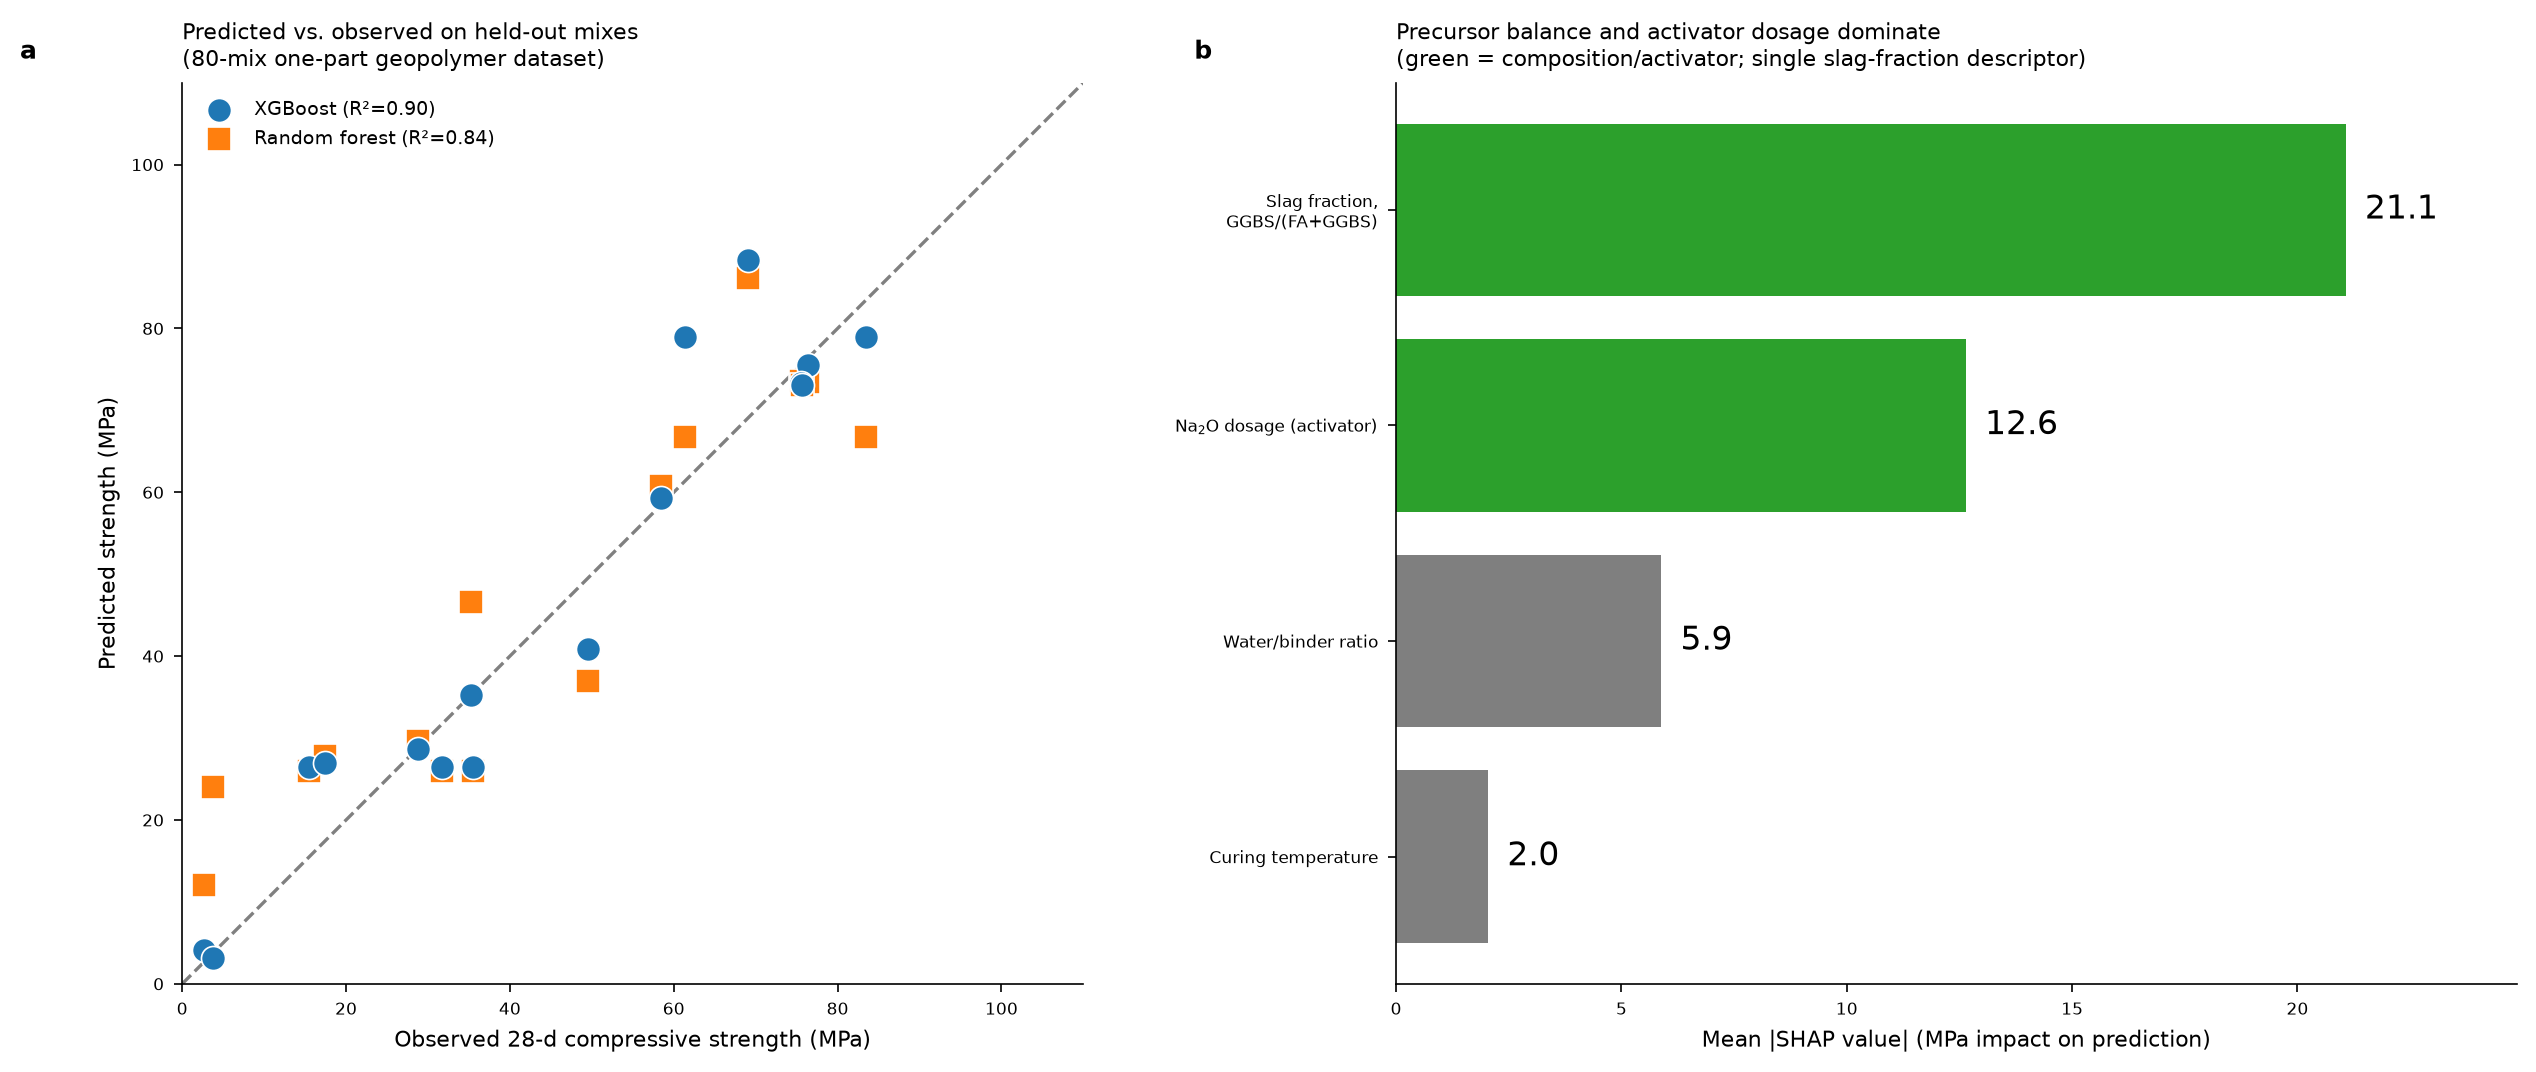
\includegraphics[width=\textwidth]{figures/figure3_ml_results.png}
\caption{ML demonstration on the 80-mix one-part geopolymer dataset. (\textbf{a}) Predicted vs.\ observed 28-day compressive strength for the two leading models on held-out data ($n = 16$); dashed line is parity. (\textbf{b}) SHAP mean absolute feature importance from the XGBoost model, computed on the re-engineered feature set in which the collinear fly-ash/GGBS pair is collapsed to a single slag fraction. The precursor balance and Na\textsubscript{2}O activator dosage (green = composition/activator) dominate the prediction.\label{fig3}}
\end{figure}

\subsection{Interpretation via SHAP}\label{sec:shap}

A feature-engineering choice precedes the interpretation. In this dataset the fly-ash and GGBS contents are near-perfectly anti-correlated (Pearson $r = -0.99$; 72 of 80 mixtures have fly-ash $+$ GGBS $= 100\%$, with a secondary component filling the balance in the remaining eight), so they carry a single compositional degree of freedom, not two. Attributing importance separately to ``fly-ash content'' versus ``GGBS content'' under such collinearity is unstable and not independently meaningful. We therefore collapse the precursor axis to one descriptor, the \textbf{slag fraction} GGBS/(fly-ash + GGBS), and compute SHAP on that re-engineered four-feature model; the collinearity is removed by construction rather than merely flagged.

TreeSHAP applied to the re-engineered XGBoost model quantifies each descriptor's mean absolute impact on the predicted strength (Figure 3b). Composition and activator terms dominate, exactly as geopolymer chemistry predicts: the slag fraction is the single largest contributor (mean |SHAP| = 21.1 MPa), followed by Na\textsubscript{2}O activator dosage (12.6 MPa), then water/binder ratio (5.9 MPa) and curing temperature (2.0 MPa). This ordering is mechanistically coherent---the fly-ash/GGBS balance sets the calcium and aluminosilicate supply that governs gel formation, and the Na\textsubscript{2}O dosage controls the alkalinity that drives dissolution and condensation---and it reproduces the sensitivity analysis reported by the dataset's original authors~\cite{ref27}, who identified alkaline dosage and slag content as the strongest levers on one-part geopolymer strength. That the model recovers this structure from held-out data, rather than being told it, is the point: an interpretable model does not merely predict strength, it tells the formulator which levers dominate and in which direction to turn them. For one-part geopolymers specifically, SHAP flags the solid-activator Na\textsubscript{2}O dosage as second only to the precursor balance---directly actionable guidance for tuning a just-add-water mix. The narrow tier occupied by curing temperature reflects the dataset's emphasis on ambient and near-ambient curing, the regime most relevant to field deployment. Extending this same analysis to multi-property targets (durability, thermal resistance, shielding) is exactly the wide-range curation that Section 5 prescribes.

\section{An AI-Assisted Design Framework for Multifunctional One-Part Geopolymers}
The demonstration generalizes into a closed-loop framework with five stages (Figure~\ref{fig4}). Before describing them, we state plainly what is \emph{demonstrated} versus \emph{proposed}, since the two must not be conflated. Section~4 demonstrates stages 1--2 in full (a curated 80-mix dataset and chemically motivated feature engineering, including the slag-fraction descriptor) and demonstrates stages 3--4 \emph{for the single target of compressive strength} (one interpretable model plus SHAP-based interpretation). It does \textbf{not} demonstrate multi-target modelling, formal multi-objective optimization, or the experimental active-learning loop; those are the framework's proposed extensions and remain future work. Figure~\ref{fig4} marks this boundary explicitly. With that scope fixed: \textbf{(1) Data curation:} assemble mixture descriptors and multi-property targets from the literature and in-house experiments into a standardized, FAIR-compliant database, explicitly recording precursor source, activator chemistry, curing, and---crucially---functional properties beyond compressive strength. \textbf{(2) Feature engineering:} encode composition as chemically meaningful descriptors (oxide ratios, reactive-phase fractions, silica modulus) rather than raw masses, improving transferability across precursor sources. \textbf{(3) Multi-target modelling:} train interpretable models not only for strength but for workability, setting time, durability, and functional targets (ductility, thermal resistance, shielding effectiveness), embracing the multi-objective nature of real design---early examples already predict freeze--thaw resistance and fibre-reinforced ductility of one-part systems~\cite{ref29,ref32,ref35}. \textbf{(4) Interpretation and optimization:} use SHAP and partial-dependence analysis to extract design rules~\cite{ref38}, then apply multi-objective optimization (e.g., Bayesian optimization or genetic algorithms over the trained surrogates) to propose candidate formulations on the performance Pareto front. \textbf{(5) Experimental validation and active learning:} synthesize and test the highest-value candidates, feed results back into the database, and iterate---each cycle sharpening the model where it is most uncertain. This loop converts one-part geopolymer development from serial trial-and-error into a guided search, and because it is built on interpretable models it yields transferable design knowledge, not just point predictions.

\begin{figure}[H]
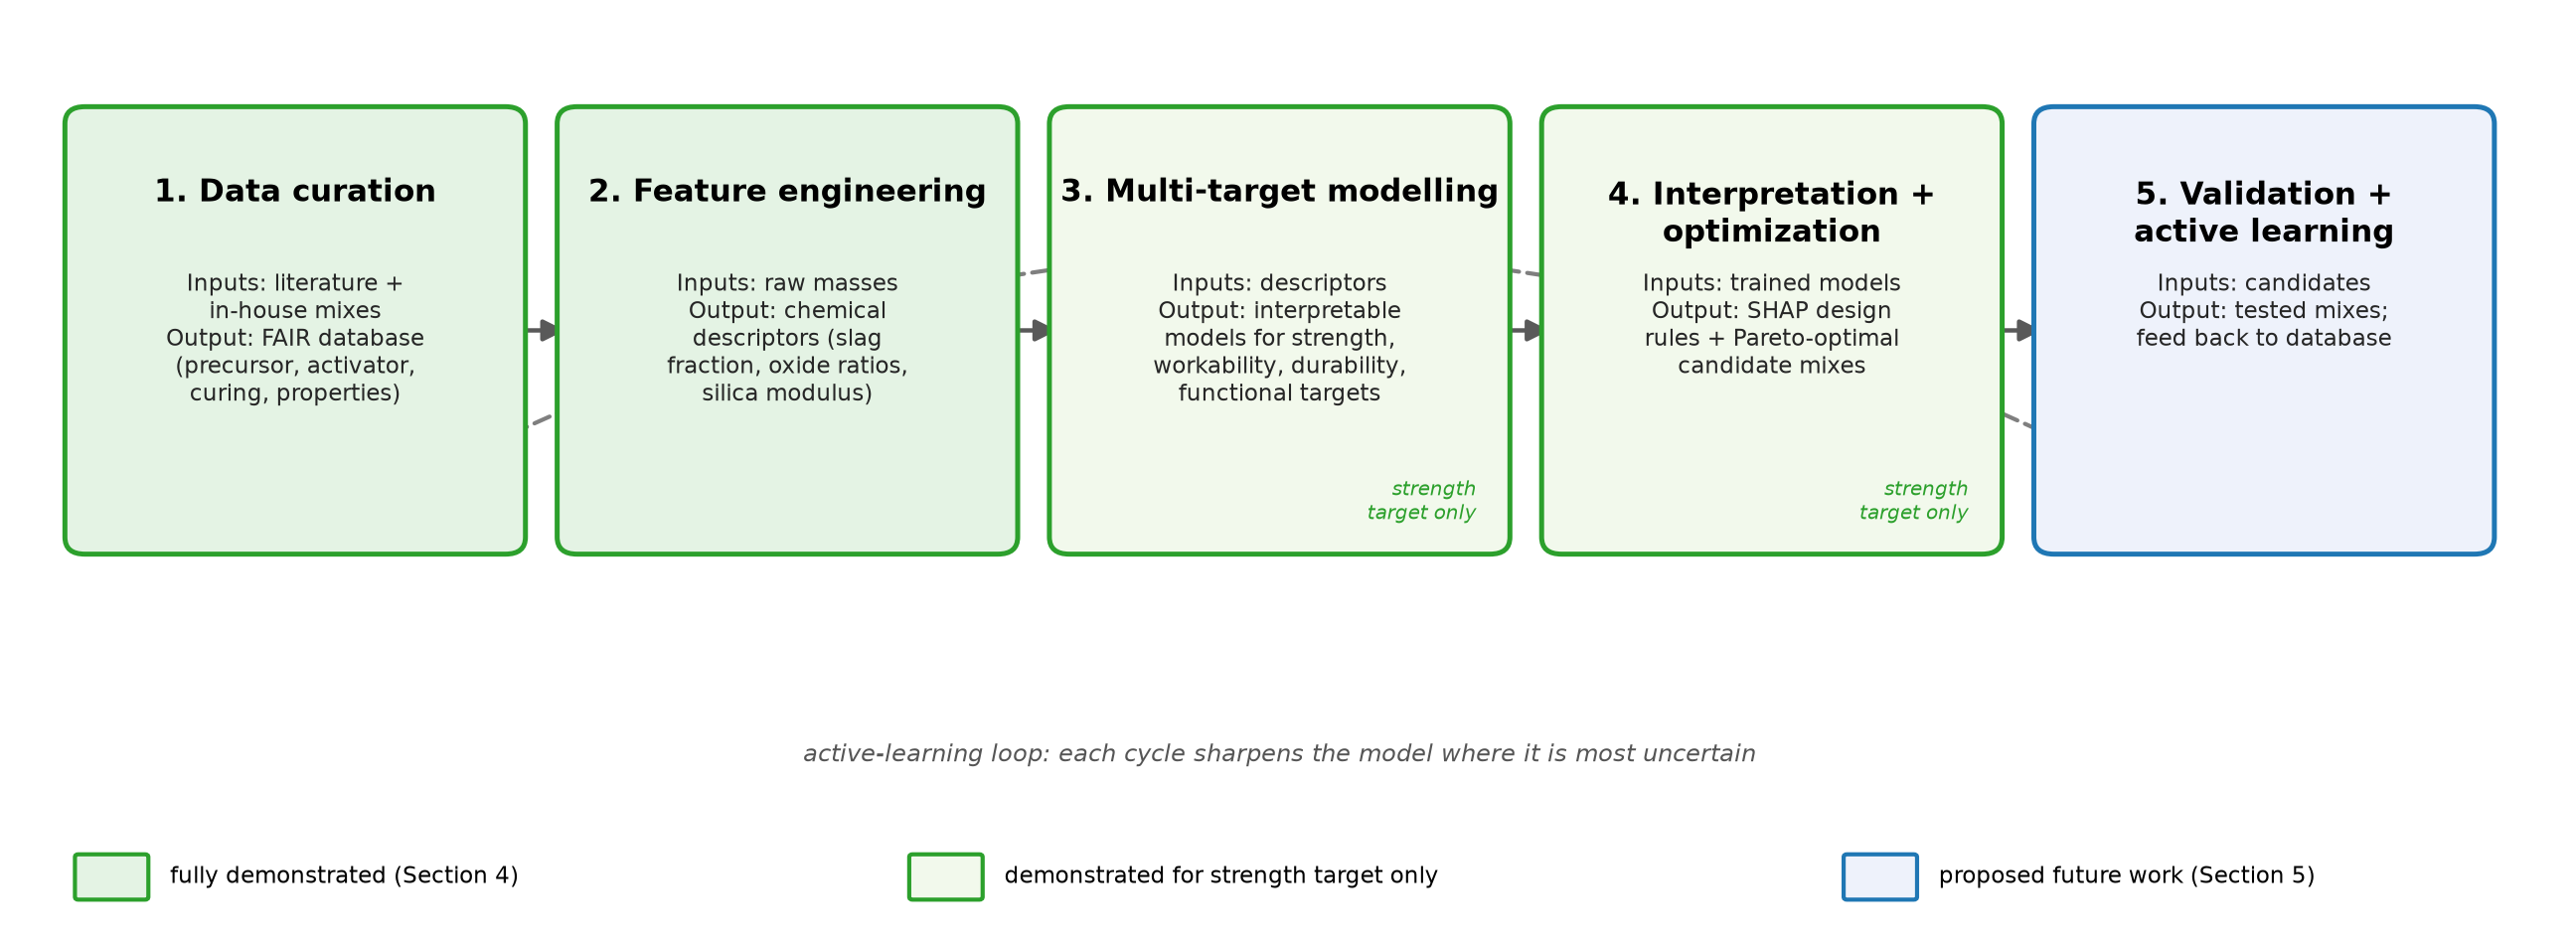
\includegraphics[width=\textwidth]{figures/figure4_framework.png}
\caption{The five-stage AI-assisted design framework, with inputs and outputs at each stage and an active-learning feedback loop. Shading distinguishes what this work demonstrates from what it proposes: stages 1--2 are demonstrated in full; stages 3--4 are demonstrated for the compressive-strength target only (badged); stage 5 and the multi-target/optimization extensions are proposed future work.\label{fig4}}
\end{figure}

\section{Limitations}
The strength of the conclusions is bounded by the demonstration's scope, which we state plainly. \textbf{(i) Dataset size.} Eighty mixtures is small for machine learning; individual LOSO folds are correspondingly noisy, and the models should be read as an illustrative benchmark, not a production predictor. \textbf{(ii) Literature-derived heterogeneity and source bias.} The data pool twelve studies with differing raw materials, mixing protocols, and testing practices; source-study effects are real---which is precisely why we evaluate by leave-one-source-out---but they also limit how far any single trained model transfers. \textbf{(iii) Feature collinearity.} The fly-ash and GGBS contents are near-perfectly anti-correlated ($r = -0.99$); we mitigate this by modelling a single slag-fraction descriptor, but the precursor axis remains a single degree of freedom in these data and cannot be resolved into independent fly-ash and slag effects. \textbf{(iv) Strength-only target.} Only 28-day compressive strength is modelled; the durability, ductility, thermal, shielding, and blast/ballistic properties invoked by ``multifunctional'' and ``defense'' framing are reviewed and built into the proposed framework but are not modelled here for want of comparable open data. \textbf{(v) Paste-level data.} The mixtures are geopolymer pastes, not concretes; aggregate, scale, and structural effects are not represented. \textbf{(vi) No experimental validation.} No new specimens were synthesized or tested; the active-learning loop of Section~5 is proposed, not executed. These limitations motivate the framework rather than undercut it: each is a specific target for the data curation, multi-target modelling, and validation stages the framework prescribes.

\section{Conclusions}
One-part geopolymers are among the most field-deployable low-carbon binder classes available, well suited to the defense and civil-infrastructure settings where liquid-activator handling is impractical. Their formulation space, however, is too large and too strongly interacting for trial-and-error development. This paper has reviewed the materials science of one-part geopolymer composites and, on a published 80-mix one-part geopolymer dataset, demonstrated that interpretable machine learning predicts \textbf{28-day compressive strength}---and only that property---with useful accuracy: a held-out test R\textsuperscript{2} = 0.90 that, under the more reliable leave-one-source-out test of transfer to a new laboratory, settles to XGBoost R\textsuperscript{2} = 0.61, well above a linear baseline (0.36). After collapsing the collinear fly-ash/GGBS pair to a single slag-fraction descriptor, SHAP recovers mechanistically coherent design rules (the precursor balance and the solid activator's Na\textsubscript{2}O dosage as the dominant strength levers). We stress the boundaries of this evidence: it is strength-only, at paste level, on 80 literature-pooled mixtures, and it does not yet substantiate the durability, ductility, thermal, shielding, or blast/ballistic performance that ``multifunctional'' and ``defense'' applications ultimately demand. Those targets are the subject of the proposed---not demonstrated---AI-assisted design framework (Section~5). The principal opportunity revealed by our bibliometric analysis is nonetheless clear: although ML for geopolymer strength prediction is now well established, the great majority of that work addresses conventional two-part mixes and compressive strength alone, leaving the one-part and multifunctional design space comparatively underexplored. Extending interpretable, multi-target data-driven design toward field-deployable multifunctional one-part composites is a tractable and high-impact direction, and the framework and worked strength example here are offered as a concrete first step toward it.

\vspace{6pt}

\authorcontributions{Conceptualization, V.N. and S.A.; methodology, V.N. and S.E.; software, V.N.; validation, S.A. and S.E.; formal analysis, V.N. and S.E.; investigation, V.N. and S.A.; resources, S.A.; data curation, V.N.; writing---original draft preparation, V.N.; writing---review and editing, all authors; visualization, V.N.; supervision, S.A. and S.E.; project administration, V.N. All authors have read and agreed to the published version of the manuscript.}

\funding{This research received no external funding.}

\dataavailability{The 80-mix one-part geopolymer dataset analyzed in Section~4 was compiled by Faridmehr et al. (\emph{Materials} 2023, 16, 2348; \url{https://doi.org/10.3390/ma16062348}) as Table~1 of that open-access (CC~BY) article, from which it was transcribed. All analysis code (a self-contained script reproducing every model, metric, SHAP value, and figure in Section~4), the cleaned dataset with per-mix source-study identifiers, the bibliometric corpus and screening table, and the 100-record tag-validation set are provided as supplementary material and archived at Zenodo (DOI: \url{https://doi.org/10.5281/zenodo.21136536}), corresponding to release \texttt{v1.0.0} of the public GitHub repository \url{https://github.com/vnageshwaran-de/geopolymer-ml-design}.}

\conflictsofinterest{Author S.A. is affiliated with Alchemy Geopolymer Solutions, a commercial entity active in geopolymer technology. This affiliation did not influence the study design, the selection or analysis of the (independently published, open-access) dataset, or the interpretation of results, and the authors declare no other conflict of interest. Consistent with this disclosure, the authors make no claim of deployment readiness or commercial performance for any specific formulation: the manuscript's contribution is a methodology and a strength-only worked example on published data, and any field or defense application would require the additional multi-property data, experimental validation, and independent qualification set out in Sections~5 and~6.}

\reftitle{References}

\begin{thebibliography}{999}
\bibitem{ref1}
Shahmansouri, A.A.; Yazdani, M.; Ghanbari, S.; Akbarzadeh Bengar, H.; Jafari, A.; Farrokh Ghatte, H. Artificial neural network model to predict the compressive strength of eco-friendly geopolymer concrete incorporating silica fume and natural zeolite. {\em Journal of Cleaner Production} {\bf 2021}. \url{https://doi.org/10.1016/j.jclepro.2020.123697}.
\bibitem{ref2}
Dao, D.V.; Ly, H.B.; Trinh, S.H.; Le, T.T.; Pham, B.T. Artificial Intelligence Approaches for Prediction of Compressive Strength of Geopolymer Concrete. {\em Materials} {\bf 2019}. \url{https://doi.org/10.3390/ma12060983}.
\bibitem{ref3}
Nguyen, K.T.; Nguyen, Q.D.; Le, T.A.; Shin, J.; Lee, K. Analyzing the compressive strength of green fly ash based geopolymer concrete using experiment and machine learning approaches. {\em Construction and Building Materials} {\bf 2020}. \url{https://doi.org/10.1016/j.conbuildmat.2020.118581}.
\bibitem{ref4}
Mozumder, R.A.; Laskar, A.I. Prediction of unconfined compressive strength of geopolymer stabilized clayey soil using Artificial Neural Network. {\em Computers and Geotechnics} {\bf 2015}. \url{https://doi.org/10.1016/j.compgeo.2015.05.021}.
\bibitem{ref5}
Ahmed, H.U.; Mohammed, A.S.; Faraj, R.H.; Abdalla, A.A.; Qaidi, S.M.A.; Sor, N.H.; Mohammed, A.A. Innovative modeling techniques including MEP, ANN and FQ to forecast the compressive strength of geopolymer concrete modified with nanoparticles. {\em Neural Computing and Applications} {\bf 2023}. \url{https://doi.org/10.1007/s00521-023-08378-3}.
\bibitem{ref6}
Awoyera, P.O.; Kirgiz, M.S.; Viloria, A.; Ovallos-Gazabon, D. Estimating strength properties of geopolymer self-compacting concrete using machine learning techniques. {\em Journal of Materials Research and Technology} {\bf 2020}. \url{https://doi.org/10.1016/j.jmrt.2020.06.008}.
\bibitem{ref7}
Shahmansouri, A.A.; Akbarzadeh Bengar, H.; Ghanbari, S. Compressive strength prediction of eco-efficient GGBS-based geopolymer concrete using GEP method. {\em Journal of Building Engineering} {\bf 2020}. \url{https://doi.org/10.1016/j.jobe.2020.101326}.
\bibitem{ref8}
Gomaa, E.; Han, T.; ElGawady, M.; Huang, J.; Kumar, A. Machine learning to predict properties of fresh and hardened alkali-activated concrete. {\em Cement and Concrete Composites} {\bf 2021}. \url{https://doi.org/10.1016/j.cemconcomp.2020.103863}.
\bibitem{ref9}
Peng, Y.; Unluer, C. Analyzing the mechanical performance of fly ash-based geopolymer concrete with different machine learning techniques. {\em Construction and Building Materials} {\bf 2022}. \url{https://doi.org/10.1016/j.conbuildmat.2021.125785}.
\bibitem{ref10}
Ahmad, A.; Ahmad, W.; Chaiyasarn, K.; Ostrowski, K.A.; Aslam, F.; Zajdel, P.; Joyklad, P. Prediction of Geopolymer Concrete Compressive Strength Using Novel Machine Learning Algorithms. {\em Polymers} {\bf 2021}. \url{https://doi.org/10.3390/polym13193389}.
\bibitem{ref11}
Khan, M.A.; Zafar, A.; Farooq, F.; Javed, M.F.; Alyousef, R.; Alabduljabbar, H.; Khan, M.I. Geopolymer Concrete Compressive Strength via Artificial Neural Network, Adaptive Neuro Fuzzy Interface System, and Gene Expression Programming With K-Fold Cross Validation. {\em Frontiers in Materials} {\bf 2021}. \url{https://doi.org/10.3389/fmats.2021.621163}.
\bibitem{ref12}
Dao, D.V.; Trinh, S.H.; Ly, H.B.; Pham, B.T. Prediction of Compressive Strength of Geopolymer Concrete Using Entirely Steel Slag Aggregates: Novel Hybrid Artificial Intelligence Approaches. {\em Applied Sciences} {\bf 2019}. \url{https://doi.org/10.3390/app9061113}.
\bibitem{ref13}
Nematollahi, B.; Sanjayan, J.; Shaikh, F.U.A. Synthesis of heat and ambient cured one-part geopolymer mixes with different grades of sodium silicate. {\em Ceramics International} {\bf 2015}. \url{https://doi.org/10.1016/j.ceramint.2014.12.154}.
\bibitem{ref14}
Ye, N.; Yang, J.; Liang, S.; Hu, Y.; Hu, J.; Xiao, B.; Huang, Q. Synthesis and strength optimization of one-part geopolymer based on red mud. {\em Construction and Building Materials} {\bf 2016}. \url{https://doi.org/10.1016/j.conbuildmat.2016.02.099}.
\bibitem{ref15}
Yousefi Oderji, S.; Chen, B.; Ahmad, M.R.; Shah, S.F.A. Fresh and hardened properties of one-part fly ash-based geopolymer binders cured at room temperature: Effect of slag and alkali activators. {\em Journal of Cleaner Production} {\bf 2019}. \url{https://doi.org/10.1016/j.jclepro.2019.03.290}.
\bibitem{ref16}
Ma, C.; Zhao, B.; Guo, S.; Long, G.; Xie, Y. Properties and characterization of green one-part geopolymer activated by composite activators. {\em Journal of Cleaner Production} {\bf 2019}. \url{https://doi.org/10.1016/j.jclepro.2019.02.159}.
\bibitem{ref17}
Ma, C.; Long, G.; Shi, Y.; Xie, Y. Preparation of cleaner one-part geopolymer by investigating different types of commercial sodium metasilicate in China. {\em Journal of Cleaner Production} {\bf 2018}. \url{https://doi.org/10.1016/j.jclepro.2018.08.060}.
\bibitem{ref18}
Nematollahi, B.; Sanjayan, J.; Qiu, J.; Yang, E.H. Micromechanics-based investigation of a sustainable ambient temperature cured one-part strain hardening geopolymer composite. {\em Construction and Building Materials} {\bf 2017}. \url{https://doi.org/10.1016/j.conbuildmat.2016.11.117}.
\bibitem{ref19}
Alrefaei, Y.; Dai, J.G. Tensile behavior and microstructure of hybrid fiber ambient cured one-part engineered geopolymer composites. {\em Construction and Building Materials} {\bf 2018}. \url{https://doi.org/10.1016/j.conbuildmat.2018.07.012}.
\bibitem{ref20}
Adesanya, E.; Ohenoja, K.; Luukkonen, T.; Kinnunen, P.; Illikainen, M. One-part geopolymer cement from slag and pretreated paper sludge. {\em Journal of Cleaner Production} {\bf 2018}. \url{https://doi.org/10.1016/j.jclepro.2018.03.007}.
\bibitem{ref21}
Muthukrishnan, S.; Ramakrishnan, S.; Sanjayan, J. Effect of alkali reactions on the rheology of one-part 3D printable geopolymer concrete. {\em Cement and Concrete Composites} {\bf 2021}. \url{https://doi.org/10.1016/j.cemconcomp.2020.103899}.
\bibitem{ref22}
Nematollahi, B.; Sanjayan, J.; Qiu, J.; Yang, E.H. High ductile behavior of a polyethylene fiber-reinforced one-part geopolymer composite: A micromechanics-based investigation. {\em Archives of Civil and Mechanical Engineering} {\bf 2017}. \url{https://doi.org/10.1016/j.acme.2016.12.005}.
\bibitem{ref23}
Hajimohammadi, A.; van Deventer, J.S.J. Characterisation of One-Part Geopolymer Binders Made from Fly Ash. {\em Waste and Biomass Valorization} {\bf 2016}. \url{https://doi.org/10.1007/s12649-016-9582-5}.
\bibitem{ref24}
Dong, M.; Elchalakani, M.; Karrech, A. Development of high strength one-part geopolymer mortar using sodium metasilicate. {\em Construction and Building Materials} {\bf 2020}. \url{https://doi.org/10.1016/j.conbuildmat.2019.117611}.
\bibitem{ref25}
Shah, S.F.A.; Chen, B.; Zahid, M.; Ahmad, M.R. Compressive strength prediction of one-part alkali activated material enabled by interpretable machine learning. {\em Construction and Building Materials} {\bf 2022}. \url{https://doi.org/10.1016/j.conbuildmat.2022.129534}.
\bibitem{ref26}
Chen, Q.; Hu, G.; Wu, J. Comparative study on the prediction of the unconfined compressive strength of the one-part geopolymer stabilized soil by using different hybrid machine learning models. {\em Case Studies in Construction Materials} {\bf 2024}. \url{https://doi.org/10.1016/j.cscm.2024.e03439}.
\bibitem{ref27}
Faridmehr, I.; Sahraei, M.A.; Nehdi, M.L.; Valerievich, K.A. Optimization of Fly Ash—Slag One-Part Geopolymers with Improved Properties. {\em Materials} {\bf 2023}. \url{https://doi.org/10.3390/ma16062348}.
\bibitem{ref28}
Chen, Q.; Hu, G.; Wu, J. Prediction of the Unconfined Compressive Strength of a One-Part Geopolymer-Stabilized Soil Using Deep Learning Methods with Combined Real and Synthetic Data. {\em Buildings} {\bf 2024}. \url{https://doi.org/10.3390/buildings14092894}.
\bibitem{ref29}
Yao, C.; Hu, G.; Chen, Q.; Wu, J. Prediction on the freeze-thaw resistance of a one-part geopolymer stabilized soil by using deep learning method. {\em Case Studies in Construction Materials} {\bf 2024}. \url{https://doi.org/10.1016/j.cscm.2024.e03530}.
\bibitem{ref30}
Wei, J.; Chen, K.; Yu, H.; Wang, S.; Zhang, S.; Pan, C. Analyzing the compressive strength of one-part geopolymers using experiment and machine learning approaches. {\em Journal of Building Engineering} {\bf 2024}. \url{https://doi.org/10.1016/j.jobe.2024.111429}.
\bibitem{ref31}
Nikmehr, B.; Kafle, B.; Al-Ameri, R. Performance Assessment of One-Part Self-Compacted Geopolymer Concrete Containing Recycled Concrete Aggregate: A Critical Comparison Using Artificial Neural Network (ANN) and Linear Regression Models. {\em Recycling} {\bf 2024}. \url{https://doi.org/10.3390/recycling9050073}.
\bibitem{ref32}
Hu, G.; Zhang, J.; Tang, Y.; Wu, J. Analysis on the Ductility of One-Part Geopolymer-Stabilized Soil with PET Fibers: A Deep Learning Neural Network Approach. {\em Buildings} {\bf 2025}. \url{https://doi.org/10.3390/buildings15152645}.
\bibitem{ref33}
Abdel-Mongy, M.; Iqbal, M.; Farag, M.; Yosri, A.M.; Alsharari, F.; Yousef, S.E.A.S. Artificial Intelligence Prediction of One-Part Geopolymer Compressive Strength for Sustainable Concrete. {\em Computer Modeling in Engineering \&amp; Sciences} {\bf 2024}. \url{https://doi.org/10.32604/cmes.2024.052505}.
\bibitem{ref34}
Pei, J.S.F.; Choo, C.S.; Khaerudini, D.S.; Bong, S.H.; Ong, D.E.L.; Sunarso, J. Evaluation of strength development of one-part alkali-activated materials through machine learning and thermodynamic modelling. {\em Cement and Concrete Composites} {\bf 2026}. \url{https://doi.org/10.1016/j.cemconcomp.2025.106364}.
\bibitem{ref35}
Zhang, J.; Hu, G.; Zhang, J.; Wu, J. Prediction of the Unconfined Compressive Strength of One-Part Geopolymer-Stabilized Soil Under Acidic Erosion: Comparison of Multiple Machine Learning Models. {\em Materials} {\bf 2026}. \url{https://doi.org/10.3390/ma19010209}.
\bibitem{ref36}
Meshram, A. Optimizing and Predicting Compressive Strength of One-Part Geopolymer Concrete. {\em International Journal for Research in Applied Science and Engineering Technology} {\bf 2023}. \url{https://doi.org/10.22214/ijraset.2023.53436}.
\bibitem{ref37}
Salman, A.; Alengaram, U.J.; Wan Jaafar, W.Z.; Suhatril, M.; Marafa, S.; Deboucha, W. Artificial neural network-based prediction of compressive strength in sustainable one-part GGBS/POFA-based geopolymer mortar with synthesized sodium silicates. {\em Journal of Sustainable Cement-Based Materials} {\bf 2025}. \url{https://doi.org/10.1080/21650373.2025.2597879}.
\bibitem{ref38}
Wang, Y.; Jia, Y.; Wang, C.; He, W.; Ding, Q.; Wang, F.; Wang, M.; Fang, K. Interpretation of Dominant Features Governing Compressive Strength in One-Part Geopolymer. {\em Buildings} {\bf 2025}. \url{https://doi.org/10.3390/buildings15203661}.
\bibitem{ref39}
Harika, R.; Venkateswara Rao, S.; Ramujee, K.; Keerthan, B. Analytical and experimental investigation on strength characteristics of one part geopolymer using machine learning models. {\em Asian Journal of Civil Engineering} {\bf 2025}. \url{https://doi.org/10.1007/s42107-025-01602-6}.
\bibitem{ref40}
Khalil, J.; Al-Fakih, A.; Yaseen, Z.M.; Al-Osta, M.A.; Hossain, M.R. Influence of chemical components and molar ratios on strength development of one-part alkali-activated mortar: Ensemble machine learning models. {\em Results in Engineering} {\bf 2026}. \url{https://doi.org/10.1016/j.rineng.2026.109621}.
\bibitem{ref41}
Kumar, S.; Sinha, A.K. Performance assessment of sustainable one-part alkali-activated concrete: An experimental and machine learning approach. {\em Research on Engineering Structures and Materials} {\bf 2026}. \url{https://doi.org/10.17515/resm2026-1531ma0224rs}.
\end{thebibliography}

\end{document}
